\subsection{Development Methodology}
The course compendium proposes two types of development methodologies: the sequential method \emph{Waterfall}, and the agile method \emph{Scrum}. This subsection supplies a brief introduction to these two approaches, followed by our argumentation for and against the two approaches in the case of our particular project. This subsequently followed by a conclusion as to which approach(es) we chose for our project.

\newpage
\subsubsection{Waterfall}
The Waterfall development method is a sequential design process. It is divided into clearly defined, mostly separated phases, although there often is some overlap between them.

The first phases focus on gathering requirements and writing initial documentation like design/architecture. Later phases move on to actual implementation, then testing and verification, followed by final report. Maintenance after a "completed" project is also in some cases a part of the process.

The unmodified waterfall model is shown in the following figure.

\begin{figure}[H]
\centering
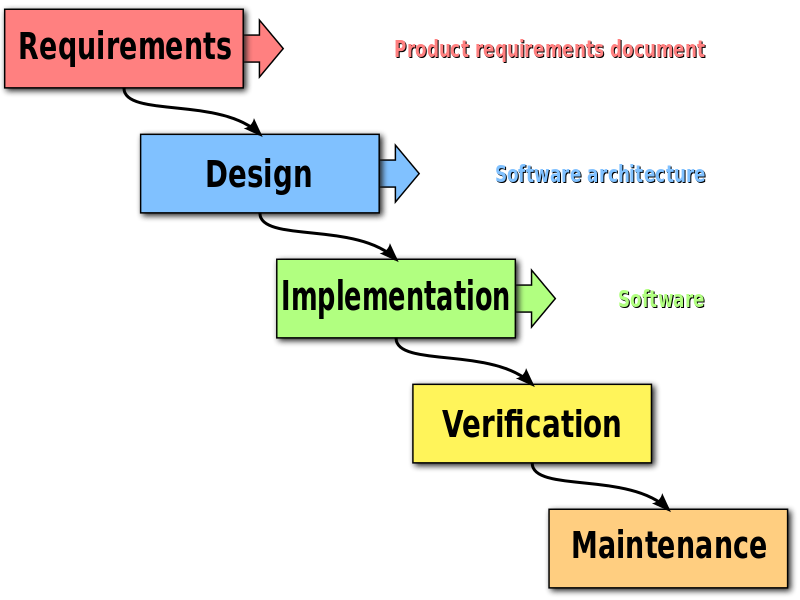
\includegraphics[width=0.8\textwidth]{images/Waterfall-model.png}
\caption{Unmodified Waterfall Model \cite{waterfallModel}}
\label{fig:Waterfall_model}
\end{figure}

\newpage
\subsubsection{Scrum}
The scrum development method is an agile approach to development. It is an iterative process consisting of several cycles or iterations. Each cycle, called a \emph{Sprint}, lasts a set length of time, typically one week to one month (7-30 days).

Within each of these cycles, most of the phases of a sequential method are covered. A sprint starts with a sprint planning session, where tasks to be completed in the sprint are planned and prioritized. The majority of the sprint consists of completing these tasks, which usually are parts of the solution that then needs to be integrated into the complete product. The sprint should result in a functioning prototype, presented to the customer at the end of the sprint to receive feedback for the next sprint, and concludes with a sprint review meeting.

The following figure depicts the typical flow in agile methods.

\begin{figure}[H]
\centering
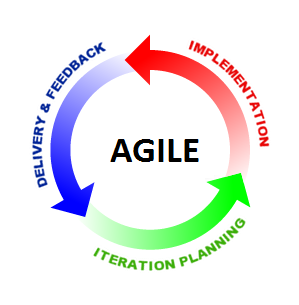
\includegraphics[width=0.8\textwidth]{images/agile-methods.png}
\caption{Agile Methods \cite{agileModel}}
\label{fig:agile_model}
\end{figure}

\subsubsection{Our choice}
Each of the proposed methods have their own advantages and disadvantages, that make each of the methods respectively a better or worse fit for our project than the other.

While the different methods have various advantageous features, not all of these are applicable to our particular project, and others are negligible.

Below we have highlighted the most important advantages and disadvantages of each method, while discussing whether or not the particular point is relevant to our project, leading to a conclusion and our choice of method. \\ \\
\emph{Waterfall} \\ \\
The following points are advantages of using the Waterfall method for projects, both in general and for ours specifically.
	\begin{itemize}
		\item Waterfall is suitable for small projects because they are manageable to fully plan. This fits our project description.
		\item It is easier to get every involved party on the same page with a thorough plan, such as provided through the Waterfall method's early phases. This is beneficial to any project, but even more so in one such as ours, where the team consists of students who may have other projects in other courses running in parallel with this.
	\end{itemize}
These next points are generally advantages of the Waterfall method, but are mostly not applicable for our project for various reasons.
	\begin{itemize}
		\item Waterfall is a good method if you know everything about the project beforehand, or are able to acquire the required information and the full project specification before the implementation phase. Due to the course schedule and the relatively limited time frame of our project, we felt we needed to start implementation earlier than a long planning and requirements phase would allow.
		\item Sequential methods require little underway feedback. This give them the edge over agile methods when access to the customer is restricted but specifications are expected to remain the same. While the specifications for our project were expected to remain unchanged, our goal was to include the customer in the process.
		\item The method supplies strong documentation as the first phases are focused entirely on creating these documents. However, while the course relies heavily on documentation, the customer had no use for most of this documentation, making this point less important for our project.
	\end{itemize}
Lastly we have the biggest disadvantage of following a sequential method, which applies to any project doing so.
	\begin{itemize}
		\item Sequential methods don't handle change to the requirements particularly well, making this approach risky in the case of the customer wishing to modify the requirements during the implementation phase.
	\end{itemize}

\emph{Scrum} \\

Advantages of agile methods such as scrum include the following:
	\begin{itemize}
		\item Agile methods support rapid production of prototypes to present to the customer. This allows for easier correction of misunderstandings, because they become apparent earlier in the process through the functioning prototypes.
		\item The method utilizes stand-up meetings, a scrum master, and optionally (and preferably) a scrum board. These things do carry overhead, but provide both the team and customer with frequent feedback, making the benefit much greater than the disadvantage of the overhead.
		
		\begin{figure}[H]
		\centering
		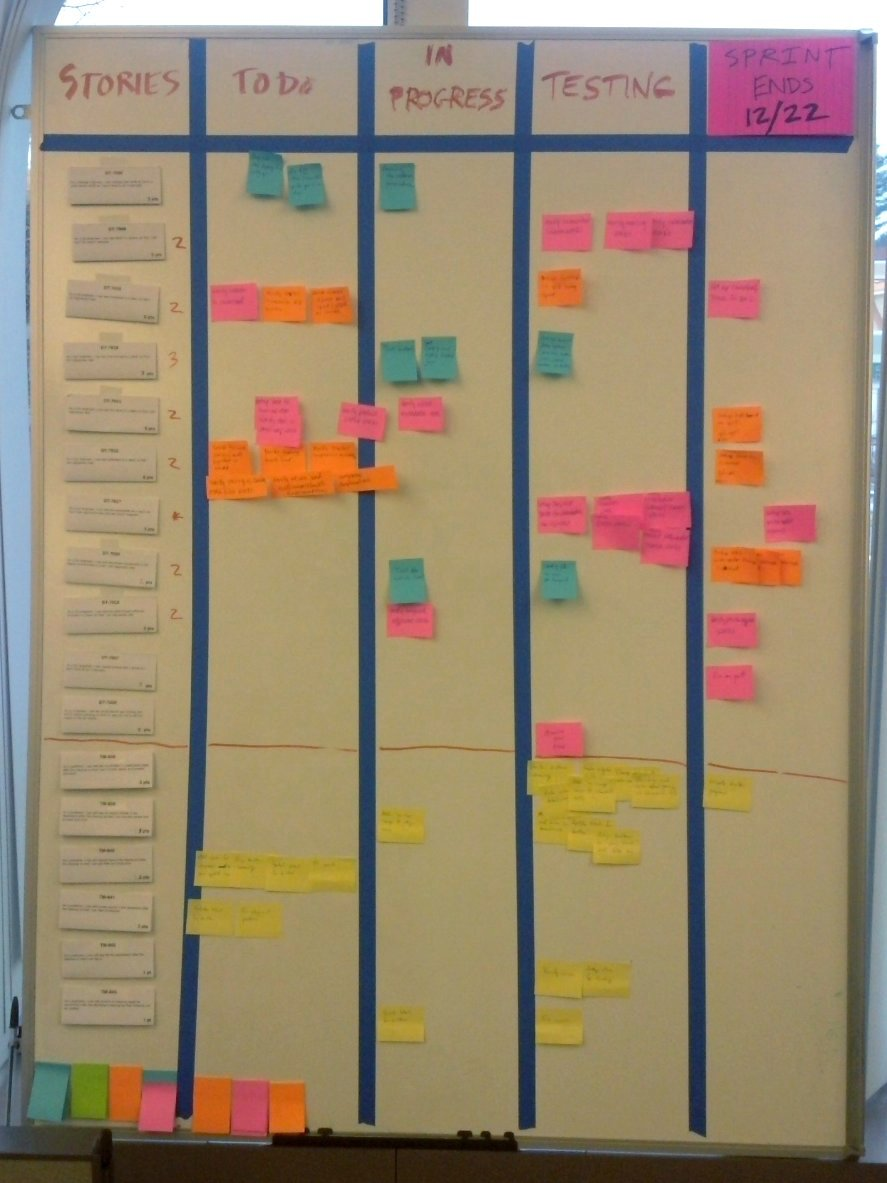
\includegraphics[width=0.8\textwidth]{images/Scrum_task_board.jpg}
		\caption{Example Scrum Board \cite{scrumBoard}}
		\label{fig:scrum_board}
		\end{figure}
		
		\item The approach is highly supported by online tools - e.g. Trello for the scrum board - that let both parties (the team and the customer) stay up-to-date on the planning and prioritization of tasks during implementation.
	\end{itemize}
While the next point generally is an advantage of agile development over a sequential process, it does contain some risks for a small project such as ours, as explained below.
	\begin{itemize}
		\item Agile methods handle change to requirements very well, due to the high level of underway involvement of the customer. The risk of weighting this point when deciding on an approach is the possibility that there simply will not be many changes, making this point irrelevant. Because we expected there to be necessary changes to the requirements and specification during the implementation, we decided this was important for our project.
	\end{itemize}
There is one major disadvantage - or rather, risk - of choosing an agile approach.
	\begin{itemize}
		\item Agile methods rely on team members - or at least the project manager - having experience with the full development process, assuming the entire project is to be completed in agile fashion.		
	\end{itemize}
There is another important point when using an agile method, which can be the deciding factor for some projects.
	\begin{itemize}
		\item Iterative approaches are heavily reliant on easy access to the customer for continuous feedback and extraction of requirements. This is okay for our project, as our customer is readily available through both e-mail and phone.
	\end{itemize}

From our analysis of the two methods, we concluded that neither were a perfect fit for every part of our project. We felt that our inexperience with projects such as this one made it too difficult to complete the entire project through an agile process, but we felt too unsure about the scope of the project to plan everything ahead and do a straight sequential process. We did, however, wish to plan an outline for the project, create a general architectural overview and gather the most important requirements before we started implementation.

This led us to a decision of employing the waterfall method, or at least something similar, for the complete process, with a relatively long period of planning before starting implementation.

The customer suggested using an agile approach for implementation because it is the same as they use. Using the same method as the customer might be beneficial to the project, as it improves communication and work flow. We decided to complete the implementation phase as an agile process, divided into two-week sprints, each consisting of a sprint planning meeting, then several days of implementation, with semi-daily stand-up meetings, and ending in a sprint review meeting and a functioning prototype.

\subsection{In Practice}
While we planned to utilize a combination of the two methods as described above, we ended up with something a little different in practice.